
\section{Selective Harmonic Elimination as dynamical system}

%


Inspired by the continuous nature of the optimization variable $ u (\tau) $ we propose in this document the formulation from the optimal control. In this way we avoid the choice of the waveform, so that the optimization problem chooses the most convenient in each case. So we look for $ \{u (\tau) \in \mathcal{U} \ | \ \forall \tau \in [0, \pi)] \} $ that has the desired Fourier coefficients.
%
We will use the fundamental theorem of differential calculus to rewrite the expression of the Fourier coefficients (\ref {an}) and (\ref {bn}) as the evolution of a dynamical system. That is to say:

\begin{gather}
    \alpha_i(\tau) = \frac{2}{\pi}\int_0^\tau u(\tau) \cos(i\tau)d\tau 
    \Rightarrow
    \begin{cases} \label{ode}
        \dot{\alpha_i}(\tau) & = \frac{2}{\pi}u(\tau)\cos(i\tau) \\  
        \alpha_i(0) & = 0       
    \end{cases}
\end{gather}

\begin{gather}
    \beta_j(\tau) = \frac{2}{\pi}\int_0^\tau u(\tau) \sin(j\tau)d\tau 
    \Rightarrow
    \begin{cases} \label{ode}
        \dot{\beta}_j(\tau) & = \frac{2}{\pi}u(\tau)\sin(j\tau) \\  
        \beta_j(0) & = 0       
    \end{cases}
\end{gather}

The evolution of the dynamical systems $ \alpha_i (\tau) $ and $ \beta_j (\tau) $ from the time $ \tau = 0 $ to $ \tau = \pi $ gives us the coefficients $ a_i $ y $ b_j $.
%
We introduce notation to refer to vectors $\bm{\alpha} = \{\alpha_i\}_{i\in\mathcal{E}_a}$ and $\bm{\beta} = \{\beta_j\}_{j\in\mathcal{E}_b}$.
%
In this way, the general SHE problem (\ref{SHEp}) can be formulated as a control problem of a dynamic system where $ \bm{\alpha} (\tau) $ and $ \bm{\beta} (\tau ) $ are the states of the system and where $ u (\tau) $ is the control variable, and whose objective will be to bring the states from the origin of coordinates to the objective vectors $ \bm{a} _T $ and $ \bm{b} _T $ in time $ \tau = \pi $.
%
In order to obtain a compact expression of the problem that simplifies our understanding of it, we will introduce notation.
%
So if we consider a problem with sets of odd numbers:
\begin{gather}
    \mathcal{E}_a = \{e_a^1,e_a^2,e_a^3,\dots,e_a^{N_a}\} \hspace{2em} \mathcal{E}_b = \{e_b^1,e_b^2,e_b^3,\dots,e_b^{N_b}\}    
\end{gather}
%
then we can define the vectors $\bm{\mathcal{D}}^\beta(\tau) \in \mathbb{R}^{N_a} $ y $ \bm{\mathcal{D}}^\beta(\tau) \in \mathbb{R}^{N_b} \ | \ \forall \tau \in (0,\pi]$ such that:
\begin{gather}
    \bm{\mathcal{D}}^\alpha(\tau) = 
    \frac{2}{\pi}
        \begin{bmatrix} 
        \cos(e_a^1\tau) \\
        \cos(e_a^2\tau) \\
        \dots           \\
        \cos(e_a^{N_a}\tau) 
    \end{bmatrix} \ \ \text{  }  \ \ 
    \bm{\mathcal{D}}^\beta(\tau) = 
    \frac{2}{\pi}
    \begin{bmatrix} 
    \sin(e_b^1\tau) \\
    \sin(e_b^2\tau) \\
    \dots           \\
    \sin(e_b^{N_b}\tau) 
    \end{bmatrix} 
\end{gather}
%
So the dynamical system can be written as:
\begin{gather}
    \begin{cases}
        \dot{\bm{\alpha}}(\tau) = \bm{\mathcal{D}}^\alpha(\tau) u(\tau) & \tau \in [0,\pi)\\
        \bm{\alpha}(0) = 0
    \end{cases} \hspace{2em}
    \begin{cases}
        \dot{\bm{\beta}}(\tau)  = \bm{\mathcal{D}}^\beta(\tau) u(\tau) & \tau \in [0,\pi) \\
        \bm{\beta}(0) = 0
    \end{cases}
\end{gather}
Compressing the notation even more we can call the total state of the system $ \bm {x} (\tau) $ to the concatenation of the states $ \bm {\alpha} (\tau) $ and $ \bm {\beta} ( \tau) $ so that:
\begin{gather}
    \bm{x}(\tau) = \begin{bmatrix}
        \bm{\alpha}(\tau) \\  \bm{\beta}(\tau)
    \end{bmatrix} \hspace{2em}
    \bm{x}_T = \begin{bmatrix}
        \bm{a}_T \\  \bm{b}_T
    \end{bmatrix} \hspace{2em}
    \bm{\mathcal{D}}(\tau) = \begin{bmatrix}
        \bm{\mathcal{D}}^\alpha(\tau) \\  
        \bm{\mathcal{D}}^\beta(\tau)
    \end{bmatrix}     
\end{gather}
%%
So for a pair of sets $ \mathcal {E} _a $ and $ \mathcal {E} _b $ we have the following associated dynamical system:
\begin{gather}
    \begin{cases}
        \dot{\bm{x}}(\tau) = \bm{\mathcal{D}}(\tau) u(\tau)  & \tau \in [0,\pi)\\
        \bm{x}(0) = {0}
    \end{cases}
\end{gather}
Then we look for a function $ u (\tau) $ such that it leads the dynamical system to the point $ \bm {x} _T $, that is, the final state $ \bm {x} (\pi) $ is $ \bm {x}_T $. Debido a que en la teoría de control es más típico llevar el sistema dinámico al origen de coordenadas desde una condición de initical no nula, realizaremos el siguiente cambio de variables: $\bm{x}'(\tau) = \bm{x}(\tau) - \bm{x}_T$. Haciendo un abuso de notación $\bm{x}'(\tau) \rightarrow \bm{x}(\tau)$  nuestro sistema dinámico se puede escribir como:

\begin{gather}
    \begin{cases}
        \dot{\bm{x}}(\tau) = -\bm{\mathcal{D}}(\tau) u(\tau)  & \tau \in [0,\pi)\\
        \bm{x}(0) = \bm{x}_T
    \end{cases}
\end{gather}

De manera que si el sistema dinámico en tiempo $\tau = \pi$ se encuentra en el origen de coordenadas, entonces los coeficientes de Fourier del control que $u(\tau)$ que le ha llevado allí son los los asociados a la condición inicial $\bm{x}_T$. 
% \begin{figure}
%     \centering
%     \begin{subfigure}[b]{0.475\textwidth}
%         \centering
%         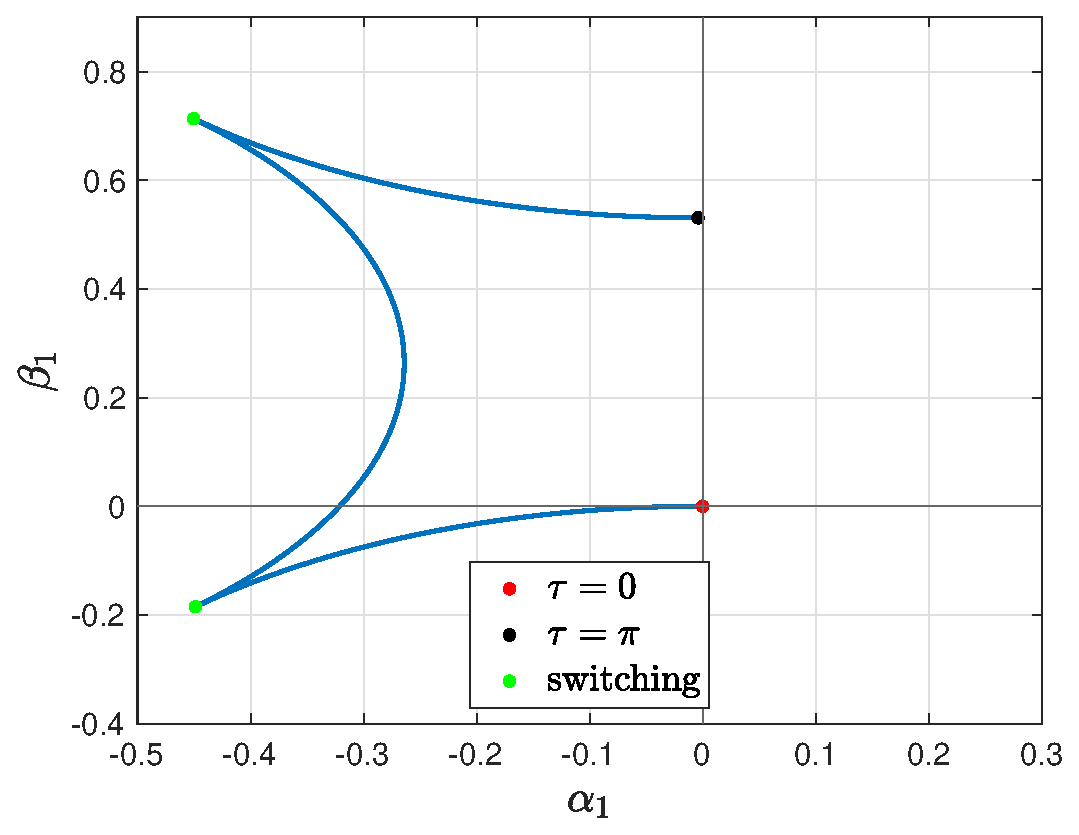
\includegraphics[width=\textwidth]{img/sys.eps}
%         \caption{Dynamical System}
%         \label{fig:sys}
%     \end{subfigure}
%     \hfill
%     \begin{subfigure}[b]{0.475\textwidth}
%         \centering
%         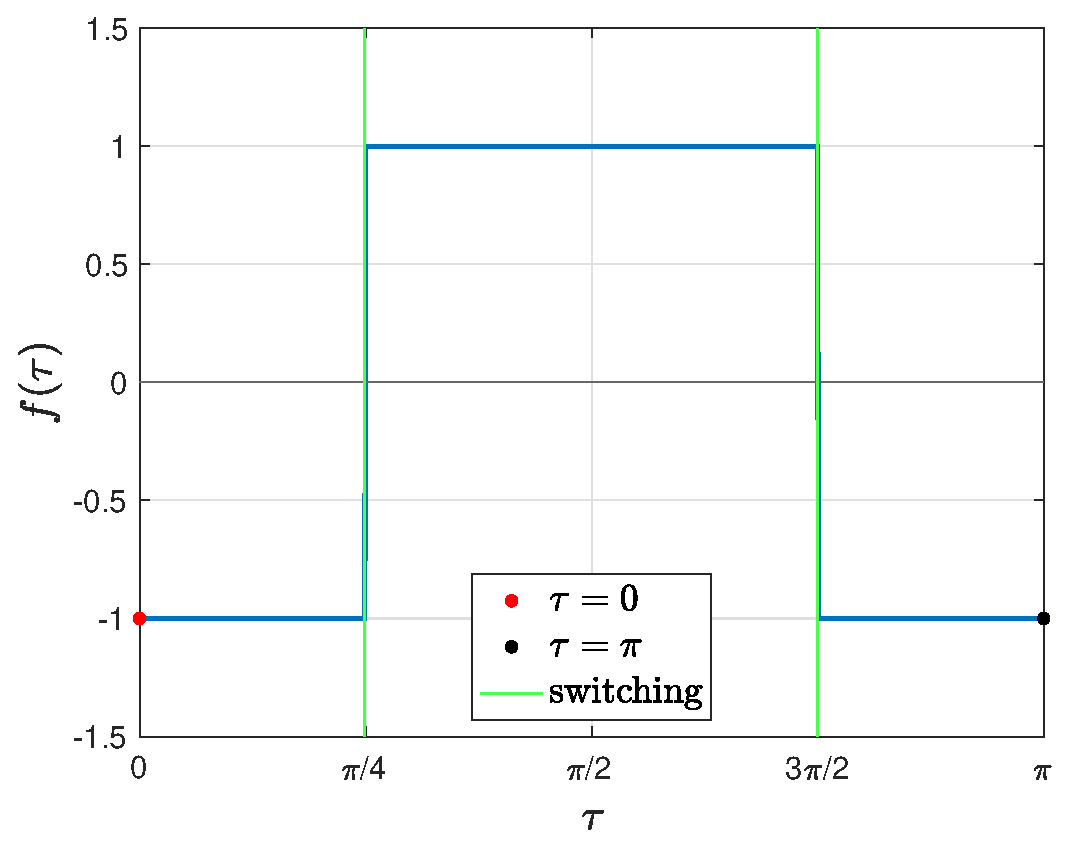
\includegraphics[width=\textwidth]{img/con.eps}
%         \caption{Control}
%         \label{fig:con}
%     \end{subfigure}
%     \caption{Mostramos el problema SHE como un sistema dinámico cuando consideramos los coeficientes de Fourier $a_1$ y $b_1$. En la figura (a) podemos ver la evolución del sistema dinámico asociado a los coeficientes de Fourier $a_1$ y $b_1$. Por otro lado, en la figura (b) podemos ver el control $u(\tau)$ que genera la trayectoria mostrada en (a).}
%     \label{syscon}
% \end{figure}